%This is a experiment example of ZhengXiaoyang's experiment report template

\documentclass[UTF8]{ctexart}
 
\usepackage{amsmath}
\usepackage{cases}
\usepackage{cite}
\usepackage{xeCJK}
\usepackage{graphicx}
\usepackage[margin=1in]{geometry}
\geometry{a4paper}
\usepackage{fancyhdr}
\pagestyle{fancy}
\fancyhf{}

\graphicspath{{picture/}}


\title{刚体转动惯量测量}
\graphicspath{{picture/}}


\title{刚体转动惯量测量预习报告}
\author{郑晓旸}
\date{\today}
\pagenumbering{arabic}

\begin{document}
%这里是文件的开头
\fancyhead[L]{郑晓旸}
\fancyhead[C]{转动惯量}
\fancyfoot[C]{\thepage}

\maketitle
\tableofcontents
\newpage

\section{实验目的}
    \begin{itemize}
        \item 通过实验加深对刚体运动定律的理解
        \item 学习两种测量刚体转动惯量的实验方法
        \item 练习用曲线拟合方法处理数据
    \end{itemize}

\section{实验仪器}
\begin{itemize}
    \item PASCO 转动及扭摆实验组件(包含支架、转动传感器、力传感器、铝盘、测试圆环、挂钩、砝码、金属丝等)
    \item 550 通用接口
    \item Capstone 软件
    \item 其它:水平尺,螺旋测微计,游标卡尺,钢卷尺,电子天平等
\end{itemize}

\section{实验原理}

    \subsection{转动定律法}
    
    如图\ref{fig:1}所示,在转动惯量测量仪上,待测物体受到重力提供的外力矩$T$和摩擦力矩$T_\mu$的作用,根据转动定律有:
    \begin{equation}
    T-T_\mu=(J+J_o+J_c)\beta \label{eq:5}
    \end{equation}
    其中$J$为待测物体的转动惯量,$J_c,J_o$分别为滑轮以及载物台等的转动惯量,$\beta$为角加速度。外力矩大小为
    \begin{equation}
    T=m(g-r_0 \beta )r_0 \label{eq:6}
    \end{equation}
    其中$m$为砝码的质量,$g$为重力加速度,$r_0$为滑轮半径。
    \\
    \begin{figure}[htbp]
        \centering
        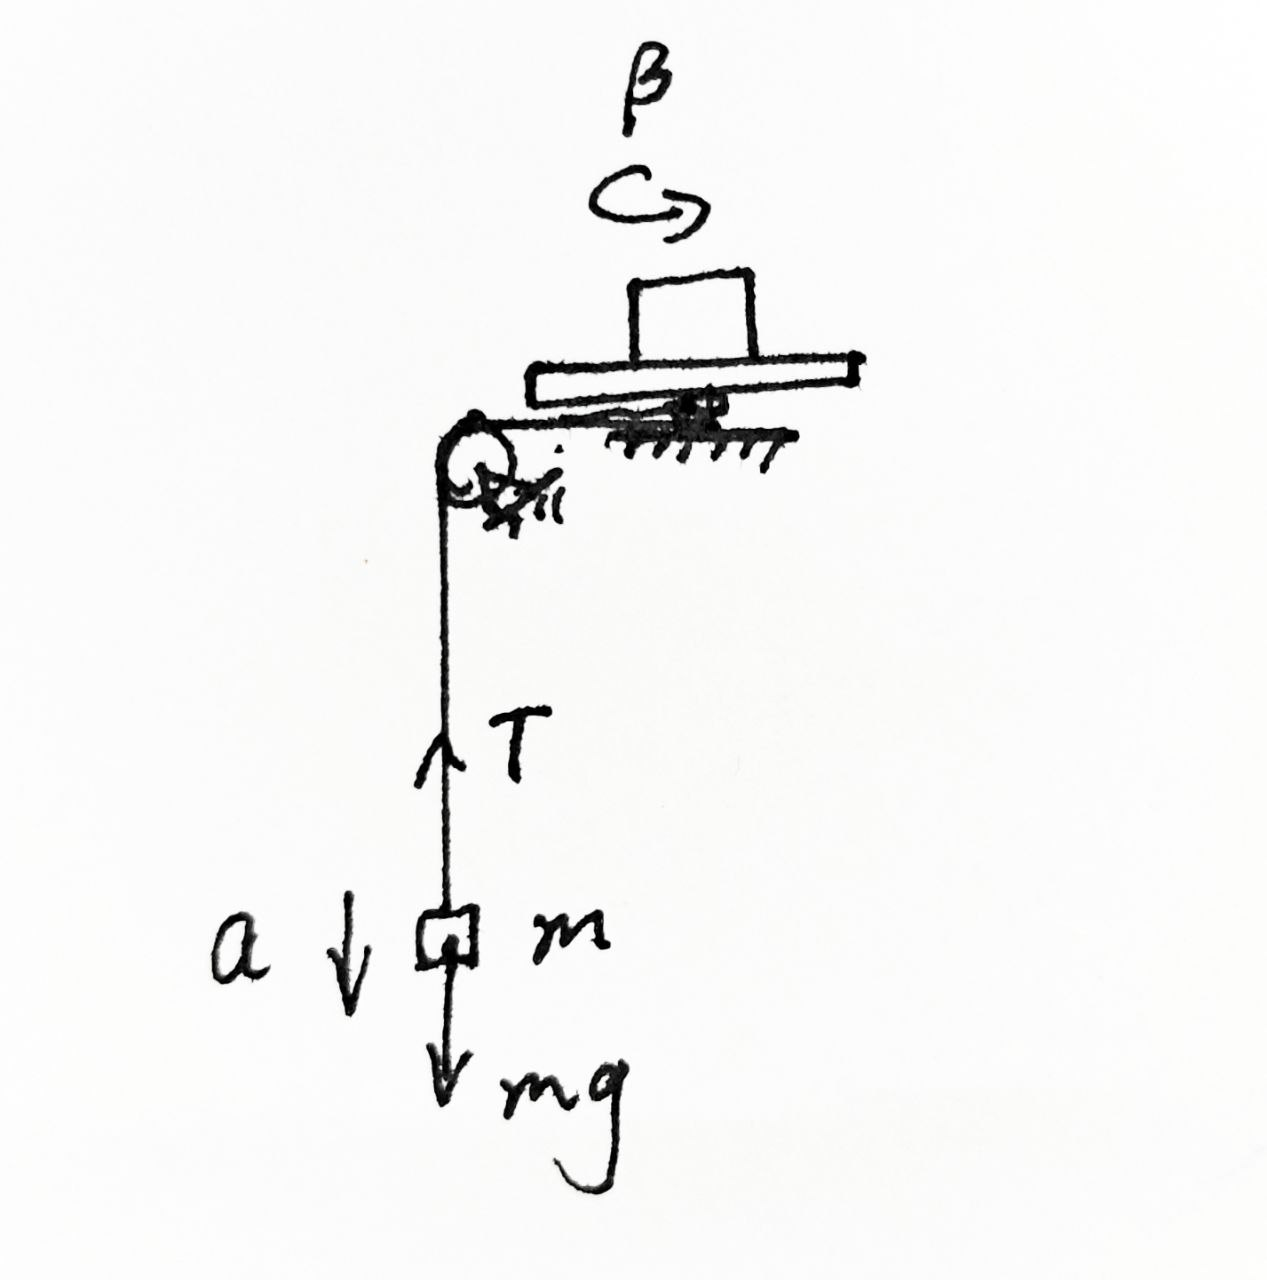
\includegraphics[width=0.4\textwidth]{rotating_platform.jpg}
        \caption{转动惯量测量仪示意图}
        \label{fig:1}
    \end{figure}
    \\
    在一系列不同重物作用下测得角加速度$\beta_i$,绘制$T$-$\beta$图像。图像应为一条斜率为$I$,截距为$-T_\mu$的直线。用最小二乘法拟合数据点,可得到总转动惯量$I$和摩擦力矩$T_\mu$。
    
    分别测量空载和负载两种情况下的总转动惯量$J_1$和$J_2$,两者之差即为待测物体的转动惯量:
    \begin{equation}
    J=J_2-J_1 \label{eq:7}  
    \end{equation}
    
    需要注意的是,由于摩擦力矩可能随转速变化,上述方法假设了$T_\mu$为常数。为尽量减小误差,应控制转速在较小的范围内变化。
    

    

    \subsection{扭摆法}
    
    将待测物体悬挂在扭丝上,偏离平衡位置后释放,在扭力矩$T$的作用下做扭摆运动。设转角为$\theta$,扭丝的扭力系数为$k$,则根据胡克定律有:
    \begin{equation}
    T=-k\theta \label{eq:8}
    \end{equation}
    由转动定律可得扭摆的运动方程为:
    \begin{equation}
    J\ddot{\theta}=-k\theta \label{eq:9}
    \end{equation}
    其中$I$为待测物体与扭摆的总转动惯量。这是一个简谐振动方程,特征角频率为
    \begin{equation}
    \omega=\sqrt{\frac{k}{J}} \label{eq:10}  
    \end{equation}
    
    实验中,先测量扭力系数$k$。在扭丝上施加一系列转角$\theta_i$,测量相应的回复力矩$T_i$,绘制$T$-$\theta$图像,如图\ref{fig:4}所示。图像应为一条过原点的直线,斜率即为$k$。
    
    然后测量扭摆周期$T$,由公式
    \begin{equation}
    \omega=\frac{2\pi}{T} \label{eq:11}
    \end{equation}
    计算特征角频率,代入公式(\ref{eq:10})即可求得总转动惯量:
    \begin{equation}
    J=\frac{kT^2}{4\pi^2} \label{eq:12}
    \end{equation}
    
    分别测量空载和负载两种情况下的扭摆周期,计算总转动惯量$J_1$和$J_2$,两者之差即为待测物体的转动惯量:
    \begin{equation}
    J=J_2-J_1 \label{eq:13}
    \end{equation}
    

    需要注意的是,由于存在空气阻力等因素,扭摆并非理想的无阻尼简谐振动,实际测得的周期会略大于理论值。为尽量减小误差,应使扭摆的初始振幅较小,并尽快测量周期。


    \section{实验过程}

    \subsection{待测圆环参数测量}
    
    \begin{enumerate}
    \item 用游标卡尺测量圆环的外径$D$,重复测量5次,每次将卡尺的位置略作变动,记录数据如表\ref{tab:1}所示。
    \item 用同样的方法测量圆环的内径$d$,重复测量5次,记录数据如表\ref{tab:1}所示。
    \item 用电子天平测量圆环的质量$m$,记录数据如表\ref{tab:1}所示。
    \item 计算外径和内径的平均值$\bar{D}$和$\bar{d}$,代入公式计算圆环的理论转动惯量$I_0$:
    \begin{equation}
    I_0=\frac{1}{8}m(\bar{D}^2+\bar{d}^2) \label{eq:14}
    \end{equation}
    \end{enumerate}
    
    \begin{table}[htbp]
    \centering
    \caption{圆环参数测量数据} \label{tab:1}
    \begin{tabular}{cccccccc}
    \hline
    测量次数 & 1 & 2 & 3 & 4 & 5 & 平均值 & 质量\\
    \hline
    外径$D$/mm &  &  &  &  &  & $\bar{D}$ & \\
    内径$d$/mm &  &  &  &  &  & $\bar{d}$ & $m$\\
    \hline
    \end{tabular}
    \end{table}
    
    \subsection{转动定律法测量转动惯量}
    
    \begin{enumerate}
    \item 将转动传感器连接到Capstone接口的通道1,选择测量角度(或角速度),线性刻度选择大滑轮,采样率设为200Hz。在采样选项中设置合适的开始和停止条件,使只记录加速过程的曲线。
    \item 设置图表,y轴为角度(或角速度),x轴为时间。  
    \item 在空载情况下,将砝码质量$m$依次设为5g、10g、15g、20g、25g、30g和35g,每次测量开始前将转盘复位,然后释放砝码,记录角度-时间(或角速度-时间)曲线。
    \item 对每条曲线进行二次多项式拟合(如果测角度)或一次多项式拟合(如果测角速度),得到角加速度$\beta_i$。
    \item 由公式(\ref{eq:6})计算各个砝码质量下的力矩$T_i$,数据记入表\ref{tab:2}。
    \item 绘制$T_i$-$\beta_i$图像,进行线性拟合,斜率即为空载情况下的总转动惯量$I_1$。
    \item 将待测圆环装到转盘上,重复步骤3-6,得到负载情况下的总转动惯量$I_2$。
    \item 由公式(\ref{eq:7})计算圆环的转动惯量$I$。
    \end{enumerate}
    
    \begin{table}[htbp]
    \centering
    \caption{转动定律法测量数据(空载)} \label{tab:2} 
    \begin{tabular}{cccccccc}
    \hline
    $m$/g & 5 & 10 & 15 & 20 & 25 & 30 & 35\\
    \hline
    $\beta_i$/(rad/s$^2$) &  &  &  &  &  &  & \\  
    $T_i$/(N$\cdot$m) &  &  &  &  &  &  & \\
    \hline
    \end{tabular}
    \end{table}
    
    \subsection{扭摆法测量转动惯量}
    
    \subsubsection{测量扭力系数}
    
    \begin{enumerate}
    \item 将转动传感器和力传感器分别连接到Capstone接口的通道1和通道2,通用采样率设为10Hz。在采样选项中设置合适的延迟启动和自动停止条件。
    \item 设置图表,y轴为力,x轴为角度。
    \item 将细线缠绕在扭摆上,逐步增大拉力,测量3次力与角度的关系,记录数据如表\ref{tab:3}所示。要求拟合直线的相关系数达到0.9999以上。
    \item 计算3次测量的扭力系数$k_i$和平均值$\bar{k}$。
    \end{enumerate}
    
    \begin{table}[htbp]
    \centering
    \caption{扭力系数测量数据} \label{tab:3}
    \begin{tabular}{ccccc}
    \hline
     & $\theta_1$/rad & $\theta_2$/rad & $\theta_3$/rad & $\theta_4$/rad\\
    \hline  
    $F_1$/N &  &  &  & \\ 
    $F_2$/N &  &  &  & \\
    $F_3$/N &  &  &  & \\
    \hline
    $k_i$/(N$\cdot$m/rad) & $k_1$ & $k_2$ & $k_3$ & $\bar{k}$\\  
    \hline
    \end{tabular}
    \end{table}
    
    \subsubsection{测量转动惯量}
    
    \begin{enumerate}
    \item 在空载情况下,手动将扭摆偏离平衡位置一小角度($<5^\circ$)并释放,记录$\theta$-$t$曲线,测量周期$T$,重复测量5次,计算平均周期$\bar{T}_1$。
    \item 由公式(\ref{eq:12})计算空载情况下的转动惯量$I_1$。
    \item 将待测圆环装到扭摆上,重复步骤1-2,得到负载情况下的平均周期$\bar{T}_2$和转动惯量$I_2$。
    \item 由公式(\ref{eq:13})计算圆环的转动惯量$I$。
    \end{enumerate}
    
    \subsection{系统摩擦力矩测量(选做)}
    
    \begin{enumerate}
    \item 在转动定律法的实验装置上,在空载情况下,给转盘一个初始角速度,记录角速度衰减到零的过程。
    \item 对$\omega$-$t$曲线进行指数拟合,得到角速度与时间的关系:
    \begin{equation}
    \omega(t)=\omega_0e^{-\frac{t}{\tau}} \label{eq:15}
    \end{equation}
    其中$\tau$为衰减时间常数。
    \item 由转动定律得到系统的摩擦力矩为:
    \begin{equation}
    T_\mu=-I_1\frac{\mathrm{d}\omega}{\mathrm{d}t}=\frac{I_1}{\tau}\omega \label{eq:16}
    \end{equation}
    \item 取$\omega$在$\omega_0/e$处的值代入公式(\ref{eq:16}),计算摩擦力矩$T_\mu$。
    \item 将测得的$T_\mu$与转动定律法中拟合得到的$T_\mu$比较。
    \end{enumerate}
    
    \section{预习思考题}
\subsection{圆环转动惯量公式的推导}
假设圆环的质量为$m$,内径为$d$,外径为$D$。取圆环的微元$\mathrm{d}m$,其到转轴的距离为$r$,则其转动惯量为
\begin{equation}
\mathrm{d}I=r^2\mathrm{d}m \label{eq:17}
\end{equation}

假设圆环的密度均匀,则微元的质量与其所占的体积成正比,有
\begin{equation}
\mathrm{d}m=\frac{m}{V}\mathrm{d}V=\frac{m}{\pi(R^2-r^2)}\cdot 2\pi r\mathrm{d}r \label{eq:18}
\end{equation}
其中$R=D/2$是圆环的外半径,$r=d/2$是圆环的内半径。
将公式(\ref{eq:18})代入公式(\ref{eq:17})并积分,得到
\begin{align}
I &= \int_{r}^{R} r^2\mathrm{d}m = \int_{r}^{R} \frac{2mr^3}{R^2-r^2}\mathrm{d}r \notag\
\\&= \frac{m}{2}\left[(R^2+r^2)-\frac{(R^2-r^2)^2}{R^2+r^2}\right] \notag\
\\&= \frac{m}{2}\left(R^2+r^2-\frac{R^4+r^4-2R^2r^2}{R^2+r^2}\right) \notag\
\\&= \frac{m}{2}\cdot\frac{2R^2r^2}{R^2+r^2} = \frac{mR^2r^2}{R^2+r^2} \label{eq:19}
\end{align}
将$R=D/2$,$r=d/2$代入,得到
\begin{equation}
I=\frac{1}{8}m(D^2+d^2) \label{eq:20}
\end{equation}
这就是圆环绕对称轴转动的转动惯量公式。
\subsection{消除摩擦力矩影响的方法}
在转动定律法和扭摆法测量转动惯量时,都需要考虑摩擦力矩$T_\mu$的影响。$T_\mu$会使测量结果偏大,因此需要想办法消除其影响。
在转动定律法中,假设$T_\mu$是常值,则有
\begin{equation}
T-T_\mu=I\beta \label{eq:21}
\end{equation}
其中$T$为外力矩,$I$为待测物体与转盘的总转动惯量,$\beta$为角加速度。
通过改变外力矩$T$的大小,测量一系列$T_i$和对应的$\beta_i$(i=1,2,3...),然后作$T_i$-$\beta_i$图,如图\ref{fig:3}所示。图像应为一条斜率为$I$,截距为$-T_\mu$的直线。用最小二乘法拟合数据点,可以得到$I$和$T_\mu$的值。由于$T_\mu$被当作拟合直线的一个参数处理,其影响可以被消除。
需要注意的是,上述方法假设$T_\mu$为常值。如果$T_\mu$与转速有关,则拟合结果会有一定误差。为了尽量减小误差,应控制转速在较小的范围内变化。
在扭摆法中,由于扭摆做简谐振动,摩擦力矩主要影响振幅的衰减,对振动周期的影响很小。因此,在测量扭摆周期时,只要振幅足够小,就可以近似认为周期不受摩擦力矩的影响。
此外,在计算转动惯量时,分别测量空载和负载两种情况下的扭摆周期,然后计算对应的转动惯量$I_1$和$I_2$,由
\begin{equation}
I=I_2-I_1 \label{eq:22}
\end{equation}
得到待测物体的转动惯量。由于空载和负载两种情况下摩擦力矩的大小近似相等,因此在式(\ref{eq:22})中相互抵消了。这也是一种消除摩擦力矩影响的方法。
当然,为了进一步减小误差,应尽量使扭摆的振幅小,周期长,以减小空气阻力等因素的影响。




\end{document}
